\chapter{Arquitectura y Diseño}
\label{Arquitectura}

VirtShell Framework es una plataforma que proporciona herramientas para la automatización y gestión de infraestructura a través del protocolo HTTP. En otros terminos, VirtShell facilita la creación, despliegue, mantenimiento y monitoreo tanto de recursos virtuales como fisicos por medio de una API REST. Esto permite que cualquier desarrollo de software con acceso a internet (sitio web, aplicación móvil, etc.) pueda utilizar VirtShell e interactuar con la infraestructura tan solo haciendo llamadas a direcciones de internet. \\
\\
VirtShell basa principalmente su funcionamiento en scripts de shell re-utilizables, que facilitan la instalación y configuraración de cualquier tipo de servidor o grandes soluciones que involucren varios recursos virtuales sin importar su tamaño. Sin embargo el lenguaje de los scripts no necesariamente debe ser el shell tambien puede interactuar con cualquier lenguaje de programación que el usuario prefiera.\\
\\
VirtShell es un framework de código abierto y bajo la licencia BSD, que permite utilizarlo para proyectos de cualquier tipo, incluso comerciales. 


% En este sentido otra ventaja importantísima es la posibilidad de crear tantos frontales como necesites con la misma API. Igual comienzas desarrollando una web, pero con la misma API podrás desarrollar también una aplicación para iOS, Android y si mañana gustas para Windows 8, Windows Phone, el próximo Windows 10, Blackberry, FirefoxOS y tantos como vengan en el futuro a encajar con tu estrategia de negocio.


% A la hora de ejecutar tu aplicación también tienes una flexibilidad mucho mayor. Las páginas del front las puedes enviar desde unos servidores y las API pueden estar alojadas en servidores independientes, tantos como necesites. Por las características de REST (principalmente no guardar estado) es indiferente qué servidor atienda cada solicitud, pues es el propio cliente el que tiene que mandar el estado al servidor, así que el balanceo de carga es mucho más simple que en aplicaciones tradicionales donde el front está mezclado con el back. También tienes la aproximación de las "micro APIs", en las que puedes dividir los procesos en diferentes servidores que atiendan a diferentes tipos de operaciones del API. 

% No mantener el estado, no requiere memoria, se pueden atender más peticiones

% -------------

\section{Características}

\begin{description}
\item [Programable] VirtShell esta orientado a realizar el aprovisionamiento de sus instancias principalmente por medio de scripts en shell, permitiendo aprovechar todas las estructuras y utilidades del lenguaje de programacion. Adicionalmente VirtShell permite extender el comportamiento del shell desplegando comandos propios que proporcionan ahorro en tiempo y en complejidad. Sin embargo, el lenguaje de shell no es de uso obligatorio, el  metodo de aprovisionamiento puede ser el de la preferencia del usuario. 
\item [Repetible] VirtShell ofrece herramientas para que los scritps de aprovisionamiento sean configurables y  puedan ser ejecutados varias veces en diferentes ambientes de desarrollo o produccion.
\item [Modular] VirtShell es un framework organizado de forma modular. Los modulos se encuentran agrupados en categorias que ofrecen las herramientas necesarias para la administracion de y aprovisionamiento de multiples recursos virtuales. De igual manera y dada las características de REST, los modulos estan diseñados para que se puedan dividir en diferentes servidores obteniendo "micro APIs", lo que permite dividir los procesos y atender diferentes tipos de operaciones del API. 
\item [Escalable] Al ser VirtShell de código abierto, el API puede modificarse, crecer facilmente y versionarse como se desee. 
\item [Seguro] VirtShell provee varias capacidades y servicios para aumentar la privacidad y el control de acceso a los diferentes recursos. Los servicios de seguridad permiten crear redes y controlar el acceso a las instancias creadas, asi como definir y administrar politicas de accesso a usuarios y permisos sobre cualquier recurso del sistema como por ejemplo scripts de creacion y aprovisionamiento.
\item [Extensible] VirtShell fue diseñado con la idea de cargar codigo dinamicamente facilmente, permitiendo extender el comportamiento del framework agregando plugins en tiempo de ejecucion.
\item [Inyección de dependencias virtuales] VirtShell adopta la idea del patrón de Inyección de Dependencias, para conseguir scripts de aprovisionamiento mas desacoplados. De esta manera facilita las configuración de las dependencias que tiene un recurso virtual de otras máquinas virtuales. Para ello, el framework permiten declarar el listado de dependencias de recursos virtuales que tiene un script aprovisionamiento encargandose del correcto acople entre los diferentes recursos virtuales.
\item [Interoperable] 
\item [Balanceable]
\end{description}

\section{Arquitectura}
VirtShell Framework consiste de caracteristicas organizadas en 12 modulos. Estos modulos son agrupados en Seguridad, Administracion y Aprovisionamiento. Estos elementos se usan de manera separada pero trabajan juntos para proveer la informacion necesaria para que los agentes realicen su trabajo en los hosts que albergaran los recursos virtuales, como se muestra en la figura. \\

\begin{figure}
	\caption{Overview of the VirtShell Framework}
	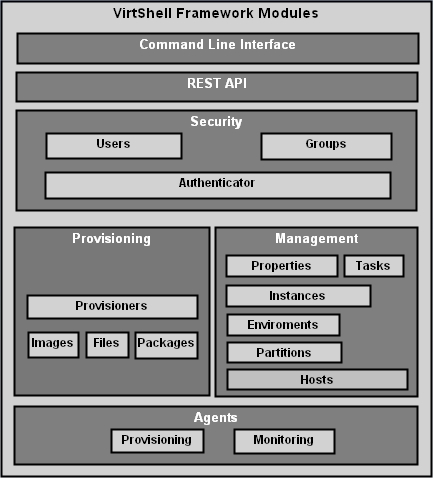
\includegraphics[width = 0.8\textwidth]{../architecture/v1/diagrams/framework}
\end{figure}

Las siguientes secciones detallan los módulos disponibles para cada característica. 

\subsection{Security}
El modulo de seguridad consisten en los modulos de usuarios, grupos y el modulo de autenticacion. El control de los usuarios y grupos es un elemento clave en la administración del framework.\\
\\
Los Usuarios pueden ser personas reales, es decir, cuentas ligadas a un usuario físico en particular o cuentas que existen para ser usadas por aplicaciones específicas.\\
\\
Los Grupos son expresiones lógicas de organización, reuniendo usuarios para un propósito común. Los usuarios dentro de un mismo grupo pueden leer, escribir o ejecutar los recursos que pertenecen a ese grupo.\\
\\
El modulo de autenticación soporta el proceso por el cual cuando un usuario se presenta a la aplicación puede validar su identidad es, de hecho, quien decide si tiene permiso para ingresar al sistema y el nivel de acceso a un recurso dado. En el capitulo 4 se detalla el proceso de autenticacion y autorizacion.

\subsection{Managment}



\subsection{Provisioning}

\subsection{Agents}


